\section{Исследование и построение решения задачи}
\label{sec:Chapter3} \index{Chapter3}

% Требуется разбить большую задачу, описанную в постановке, на более мелкие
% подзадачи. Процесс декомпозиции следует продолжать до тех пор, пока подзадачи
% не станут достаточно простыми для решения непосредственно. Это может быть
% достигнуто, например, путем проведения эксперимента, доказательства теоремы
% или поиска готового решения.

В данном разделе будут более подробно рассмотрены идеи, которые были разработаны в ходе исследования решения задачи. Реализации данных идей посвящена следующая глава. 

\subsection{Проблема ленивых вычислений}

Как уже обсуждалось во введении, ленивые вычисления используются для экономии времени на проведении вычислений, результаты которых заведомо не будут использованы программой в дальнейшем. Не смотря на очевидные преимущества ленивых вычислений, в некоторых случаях строгое следование этому правилу может препятствовать векторизации инструкций, что в свою очередь могло бы дать прирост производительности.

Например, на рисунке ~\ref{lazyeval} векторизация двух обращений в память не может быть произведена, поскольку в зависимости от результата первого условия вычисление второго может не произойти. Векторизация такого участка кода может привести к доступу к данным, которые по стандарту языка не должны загружаться. В свою очередь это может привести к ошибке отказа доступа в данный участок памяти (рис. ~\ref{arr1}).

\begin{figure}[!htb]
    \centering
    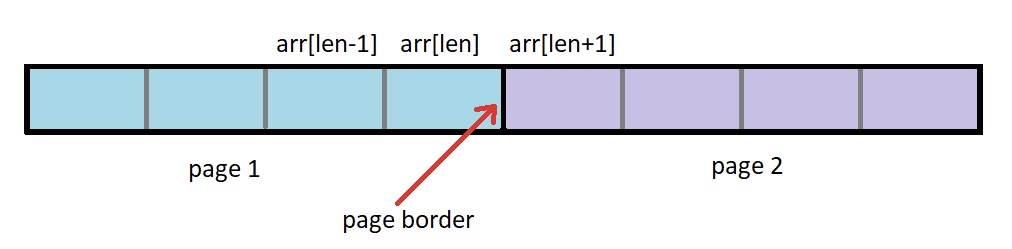
\includegraphics[scale=0.35]{arrinpage.jpeg}
    \caption{Пример ситуации, когда элементы массива лежат в двух страницах в памяти}
    \label{arr1}
\end{figure}

Данную проблему можно решить благодаря страничной организации памяти. Концепция такой памяти гарантирует наличие данных в пределах страницы, даже если те не были использованы во время исполнения программы. В данной работе предлагается использовать знание о страничной организации памяти и о минимальном размере страницы для векторизации таких выражений. Для этого необходимо проверить, что оба обращения в память находятся в одной странице, тем самым избежав ситуации обращения в не выделенную память при попытке их объединения (рис. ~\ref{arr2}).

\begin{figure}[!htb]
    \centering
    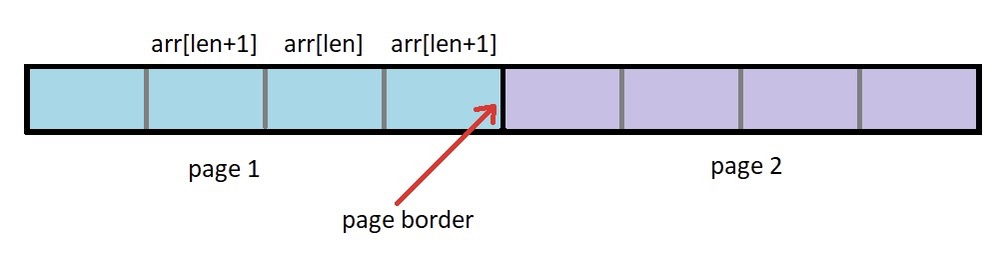
\includegraphics[scale=0.35]{arrinpage2.jpeg}
    \caption{Пример ситуации, когда элементы массива лежат в одной странице в памяти и могут быть векторизованы}
    \label{arr2}
\end{figure}

\subsection{Векторизация без использования SIMD}

В данной работе было решено ограничиться использованием скалярных операций, поскольку векторизация ленивых вычислений накладывает некоторые ограничения в виде потребности векторного сравнения и т.п. Чтобы решить данную проблему было предложено использовать скалярные регистры, данные в которые будут загружаться по секциям с помощью битовых \textit{сдвигов и масок}. Пример такого механизма представлен на рисунке ~\ref{charint}.

\begin{figure}[!htb]
    \centering
    \includesvg[scale=0.9]{4chartoint1.svg}
    \caption{Пример использования скалярного типа для векторизации}
    \label{charint}
\end{figure}

В данном случае удается эмулировать параллельное выполнение за счет уменьшения количества обращений в память с использованием обычных регистров. Однако максимальный размер скалярного регистра ограничивает область применения данного подхода и позволяет в основном получать выигрыш благодаря загрузки данных, обладающих маленьким размером типа. На рисунке ~\ref{charint} представлен пример загрузки 4 элементов однобайтового массива типа $char$ в один элемент размера $int$. Несмотря на подобные ограничение, такой подход все еще остается выигрышным. Тем не менее, в будущем планируется избавиться от данного ограничения путем использования векторного сравнения и улучшения самого алгоритма векторизации.  
\newpage
